
\begin{frame}[t]{Motivación del proyecto}

    \begin{onlyenv}<1>
    En el Laboratorio de Electrónica Cuántica (LEC) se dispone de un microscopio SPIM

    \begin{columns}
        \begin{column}{0.5\textwidth}
            \begin{itemize}
                \item Utiliza muestras con fluoroforos
                \item Con una hoja de luz (lightsheet) ilumina un plano de la muestra por vez
                \item Disminuye el photobleaching (blanqueo de los flouroforos)
                \item Permite recostruir una imagen en 3D de la muestra
            \end{itemize}
        \end{column}
        \begin{column}{0.5\textwidth}
            \begin{figure}[H]
                \centering
                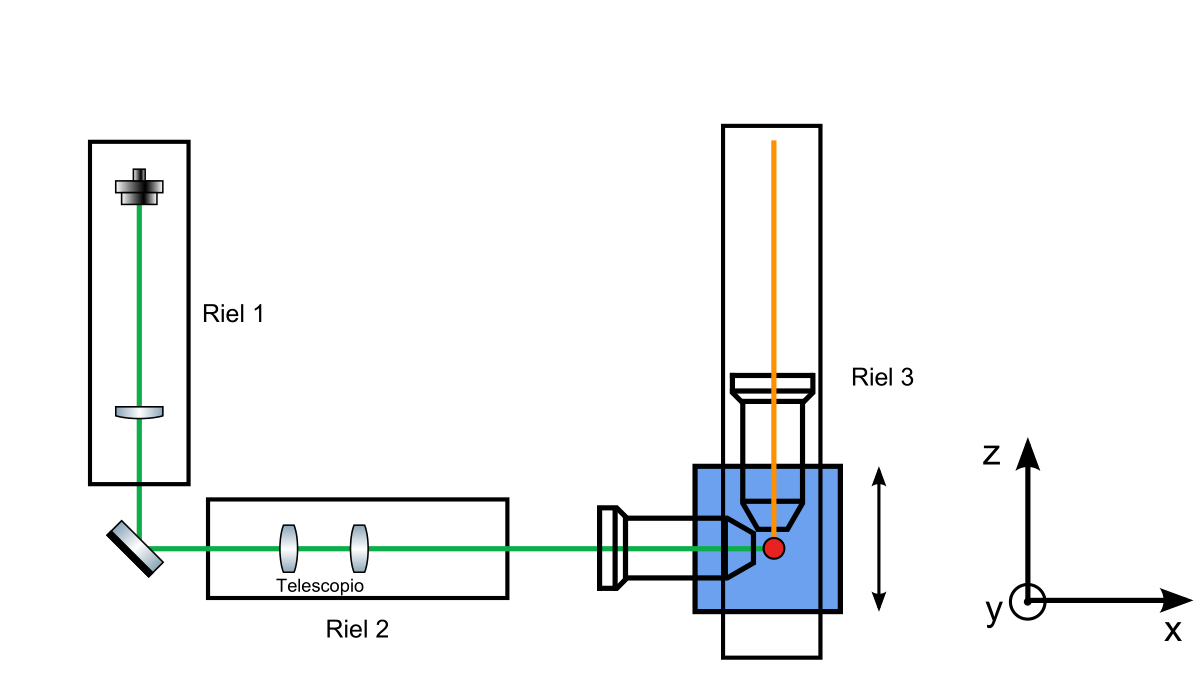
\includegraphics[width=\textwidth]{fig/spim}
                \label{fig:spim} 
            \end{figure}
        \end{column}
        \end{columns}
    \end{onlyenv}

    \begin{onlyenv}<2>
        La construcción de este microscopio requiere determinar
        \begin{columns}
            \begin{column}{0.5\textwidth}
                \begin{itemize}
                    \item Perfil del haz, que cambia el tamaño de la hoja del haz
                    \item Espectro del haz, determina los flouroforos a utilizar
                    \item Polarización del haz, que si es lineal permite hacer mediciones de anisotropía de los fluoroforos
                \end{itemize}
            \end{column}
            \begin{column}{0.5\textwidth}
                \begin{figure}[H]
                    \centering
                    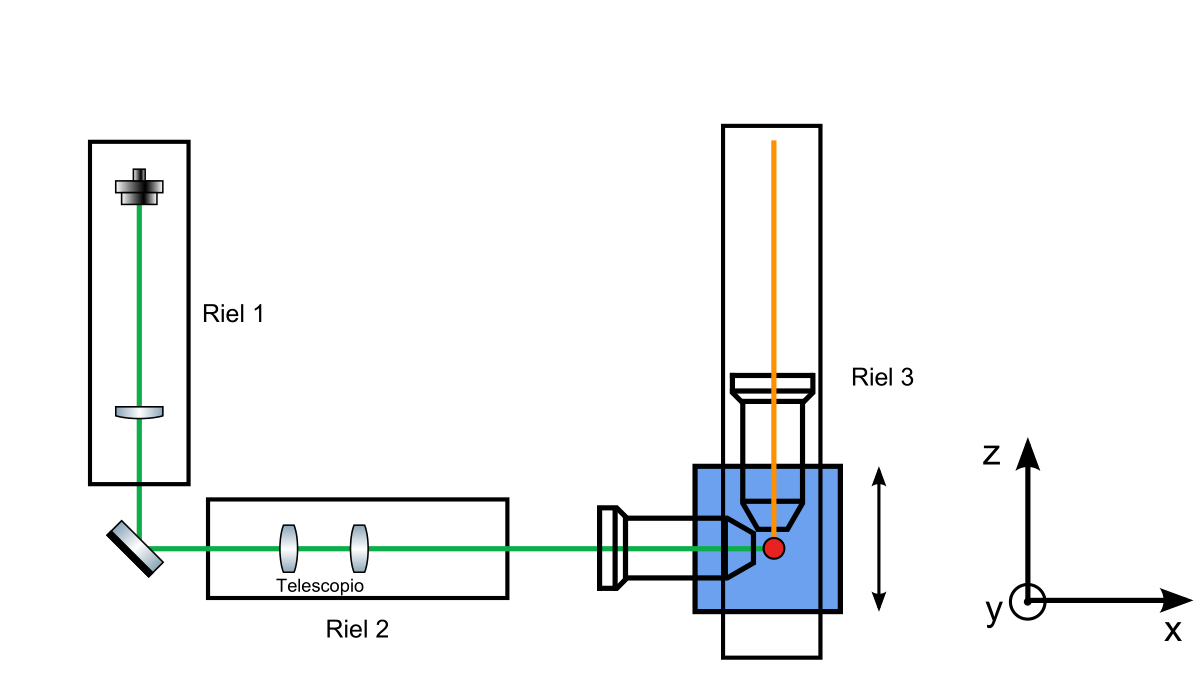
\includegraphics[width=\textwidth]{fig/spim}
                    \label{fig:spim} 
                \end{figure}
            \end{column}
        \end{columns}
        \vspace{1em}
        Para calibrar el SPIM,se construyó el siguiente instrumental portátil
        \begin{itemize}
            \item Perfilador
            \item Polarimetro
        \end{itemize}
    \end{onlyenv}

\end{frame}

